\documentclass{beamer}
\usepackage[orientation=landscape,size=a0,scale=1.4]{beamerposter}
\mode<presentation>{\usetheme{HHMI}}
\usepackage{chemformula}
\usepackage[utf8]{inputenc}
\usepackage[german, english]{babel} % required for rendering German special characters
\usepackage{siunitx} %pretty measurement unit rendering
\usepackage{hyperref} %enable hyperlink for urls
\usepackage{ragged2e}
\usepackage{tikz}
\usepackage{array,booktabs,tabularx,xspace}
\usepackage{scrextend}
\usepackage{pdfpages}
\usepackage{siunitx}

\usetikzlibrary{shapes,arrows,trees,calc,decorations.markings}

\newcolumntype{Z}{>{\centering\arraybackslash}X} % centered tabularx columns

\title{\huge Women's Coding Circle}
\author{-}
\institute{HHMI Janelia Research Campus, Ashburn, USA}

\newlength{\columnheight}
\setlength{\columnheight}{50cm}

\makeatletter
\let\@cite@ofmt\@firstofone % not \hbox
\makeatother

\setbeamertemplate{bibliography entry title}{}
\setbeamertemplate{bibliography entry location}{}
\setbeamertemplate{bibliography entry note}{}

\begin{document}
\begin{frame}
\vspace{-12cm}
\begin{columns}
	\begin{column}{.33\textwidth}
		\begin{beamercolorbox}[center,wd=\textwidth]{postercolumn}
			\begin{minipage}[T]{.95\textwidth}  % tweaks the width, makes a new \textwidth
				\parbox[t][\columnheight]{\textwidth}{ % must be some better way to set the the height, width and textwidth simultaneously
					\begin{myblock}{WCC Officers}
					    \begin{addmargin}[1em]{1em}
                            The officers are the leadership team of the WCC. Together we plan upcoming events, invite speakers and prepare coding classes.
                        \end{addmargin}
                        \begin{addmargin}[1em]{1em}
                            \vspace{1.5cm}
                            \begin{figure}
                                \centering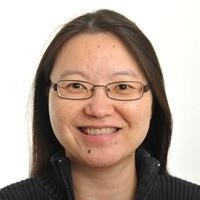
\includegraphics[width=0.3\textwidth]{img/teri.jpg}
                                \centering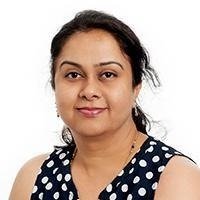
\includegraphics[width=0.3\textwidth]{img/kshama.jpg}
                                \centering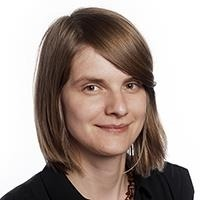
\includegraphics[width=0.3\textwidth]{img/antje.jpg}
                                \caption{Teri Ngo, Kshama Aswath, Antje Kazimiers}
                                \label{fig:workspace}
                                \vspace{1.3cm}
                            \end{figure}
                            \begin{figure}
                                \centering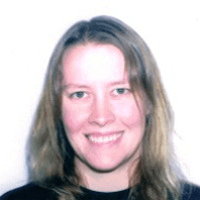
\includegraphics[width=0.3\textwidth]{img/lisa.png}
                                \centering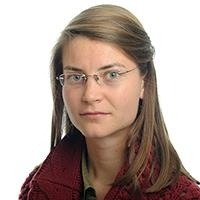
\includegraphics[width=0.3\textwidth]{img/hannah.jpg}
                                \centering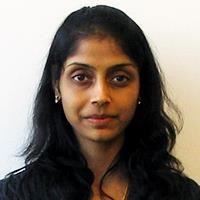
\includegraphics[width=0.3\textwidth]{img/sarada.jpg}
                                \caption{Lisa Taylor, Hannah Haberkern, Sarada Viswanathan, ..and you?}
                                \label{fig:workspace}
                                \vspace{1.3cm}
                            \end{figure}
                        \end{addmargin}
                    \end{myblock}
                    \vspace{1.25cm}
                    \begin{myblock}{Classes}
                        \begin{addmargin}[1em]{1em}
                            Our classes include running commands on the terminal, Python and \LaTeX.
                        \end{addmargin}
                    \end{myblock}\vfill
                    \vspace{1.25cm}
					\begin{myblock}{Open Source}
					    \begin{addmargin}[1em]{1em}
                            We are publishing our code on github under open source licenses like MIT or GPL.
                            Among the projects you can find there are Python and HTML classes and tutorials, presentation slides written with RevealJS,
                            a Python Flask application and Howtos, how to get started with using the command line and programming in general.
                        \end{addmargin}
                        \begin{addmargin}[1em]{1em}
                            \begin{figure}
                                \vspace{1cm}
                                \centering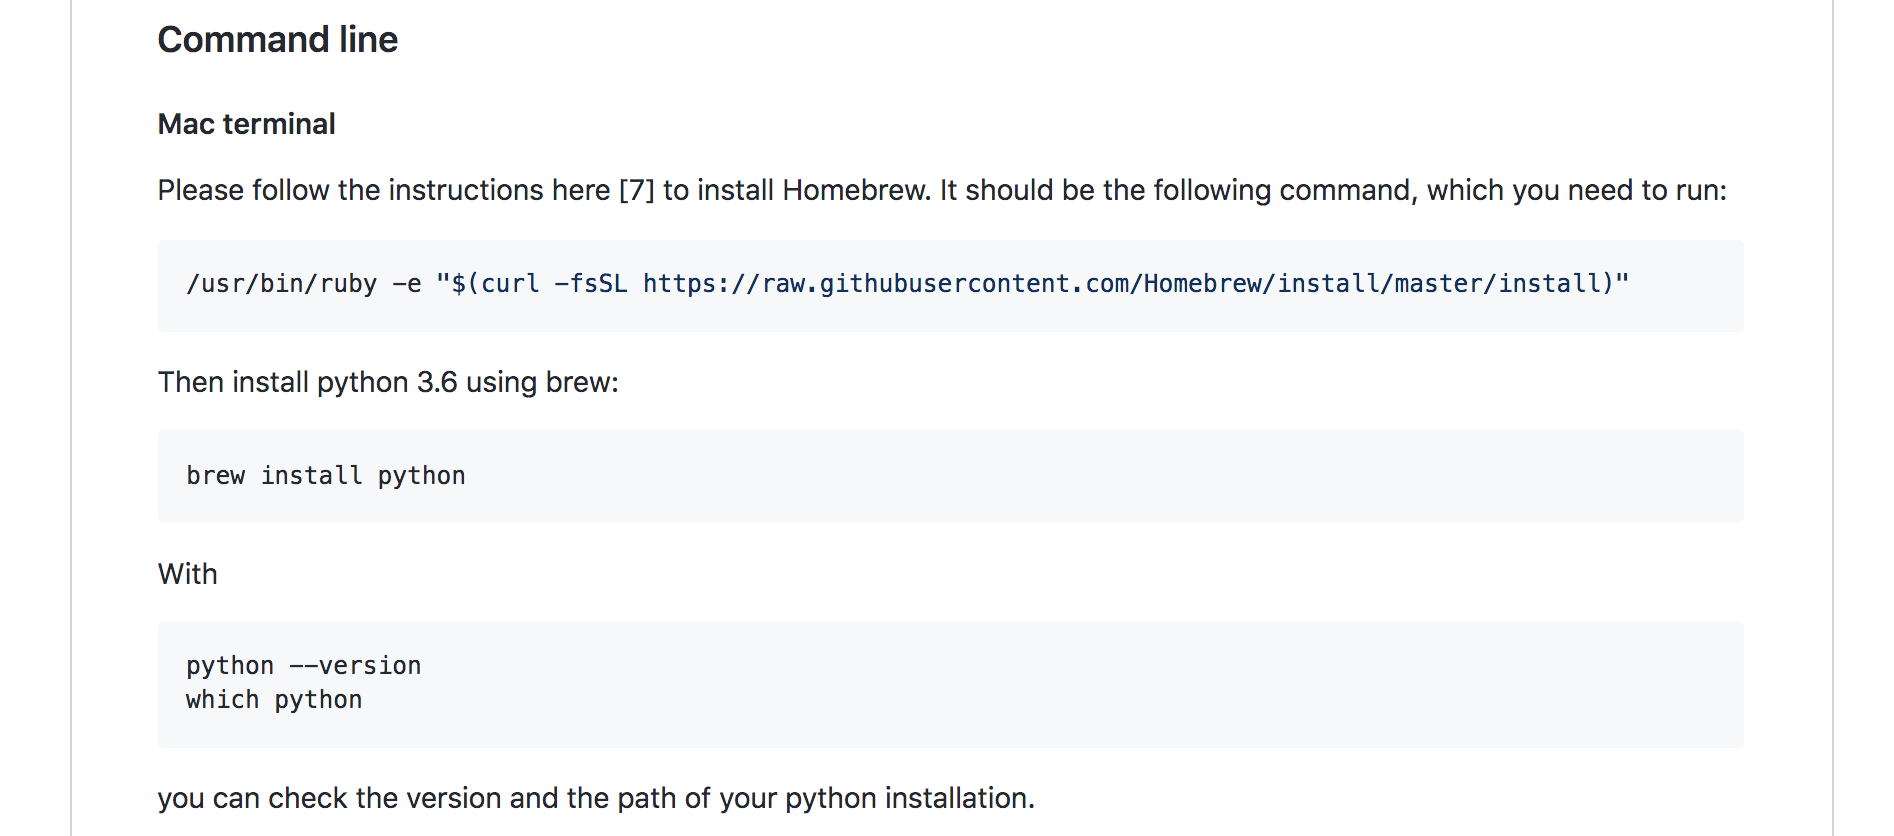
\includegraphics[width=0.59\textwidth]{img/cmd.png}
                                \vspace{1cm}
                            \end{figure}
                        \end{addmargin}
                    \end{myblock}\vfill
		}\end{minipage}\end{beamercolorbox}
	\end{column}
  \begin{column}{.33\textwidth}
		\begin{beamercolorbox}[center,wd=\textwidth]{postercolumn}
			\begin{minipage}[T]{.95\textwidth}
				\parbox[t][\columnheight]{\textwidth}{
					\begin{myblock}{What is the Women's Coding Circle?}
                        \begin{addmargin}[1em]{1em}
                            The inspiration for the WCC is a knitting circle: We meet to talk about any topics related to being a Woman in Science and and a Woman who codes.
                            We are exploring technologies, held classes, work on coding issues and share our knowledge.\newline
                            From time to time, we invite group leaders and senior scientist to learn from them, what helped them being successful during their career.
                        \end{addmargin}
                    \end{myblock}
                    \vspace{1.25cm}
                    \begin{myblock}{Our mission}
                        \begin{addmargin}[1em]{1em}
                                ..

                        \end{addmargin}
                    \end{myblock}
                    \vspace{1.25cm}
                    \begin{myblock}{TBA}
                        \begin{addmargin}[1em]{1em}
                        \end{addmargin}
                    \end{myblock}
                    \vspace{1.25cm}
                    \begin{myblock}{Want to join?}
                        \begin{addmargin}[1em]{1em}
                            We meet several times a month for a coding class, with an invited speaker to plan upcoming events. Our events are open to all women in Janelia, including spouses and children, and to all people, who identify as a woman.\newline
                            To join the club, please reach out to one of the officers, we can sign you up for our mailing list and Slack channel.
                        \end{addmargin}
                    \end{myblock}
                }
		    \end{minipage}\end{beamercolorbox}
  \end{column}
	\begin{column}{.33\textwidth}
		\begin{beamercolorbox}[center,wd=\textwidth]{postercolumn}
			\begin{minipage}[T]{.95\textwidth}
				\parbox[t][\columnheight]{\textwidth}{
					\begin{myblock}{Speakers Series}
            \begin{addmargin}[1em]{1em}
                We are inviting women in leadership roles in HHMI to our group to talk about their scientific background, mentors, role models and anything else, what helped them being successful.
            \end{addmargin}
            \begin{addmargin}[1em]{1em}
                \vspace{1.5cm}
                \begin{figure}
                    \centering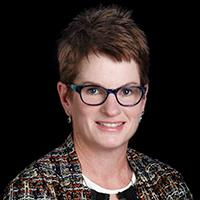
\includegraphics[width=0.45\textwidth]{img/erin.jpg}
                    \centering
\includegraphics[width=0.45\textwidth]{img/kathryn.jpg}
                    \caption{Erin O'Shea, Kathryn Brown}
                    \label{fig:workspace}
                    \vspace{1.3cm}
                \end{figure}
                \begin{figure}
                    \centering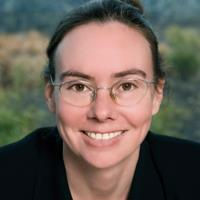
\includegraphics[width=0.45\textwidth]{img/roian.jpg}
                    \centering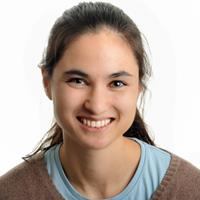
\includegraphics[width=0.45\textwidth]{img/kristin.jpg}
                    \caption{Roian Egnor, Kristin Branson}
                    \label{fig:workspace}
                    \vspace{1.3cm}
                \end{figure}
            \end{addmargin}
            \vspace{1cm}
          \end{myblock}\vspace{1.25cm}
			\begin{myblock}{TBA}
                \begin{addmargin}[1em]{1em}
                \end{addmargin}
            \end{myblock}\vspace{1.25cm}

			\begin{myblock}{TBA}
                \begin{addmargin}[1em]{1em}
                \end{addmargin}
			\end{myblock}
		}\end{minipage}\end{beamercolorbox}
	\end{column}
\end{columns}
\end{frame}
\end{document}
